\documentclass[conference]{IEEEtran}

%\vfill\eject
% https://www.sharelatex.com/blog/2013/08/07/thesis-series-pt3.html

\usepackage{hyperref}
\usepackage{graphicx}
\usepackage{lscape}
\usepackage{tipa}
\usepackage{amsmath}
\usepackage{verbatim} % for \begin{comment}
\usepackage{caption} % for subfigures
\usepackage{subcaption} % for subfigures

\begin{document}
\title{CDN Improvements with Bloom Push and DHTs}

\author{
	\IEEEauthorblockN{Lisa Peters}
	\IEEEauthorblockA{\href{mailto:lisapeters.peters@gmail.com}{lisapeters.peters@gmail.com}}
	\and
	\IEEEauthorblockN{Nate Woods}
	\IEEEauthorblockA{\href{mailto:me@bign8.info}{me@bign8.info}}
}
\IEEEspecialpapernotice{Gianforte School of Computing at Montana State University}

\maketitle
\thispagestyle{plain}
\pagestyle{plain}

\section{Introduction}\label{sec:intro}
CDNs are ubiquitous throughout the infrastructure of the internet, being used by many companies for the purpose of serving content to clients. For the average user, speed is the most important in terms of performance. As content providers, CDNs need to have very fast response times to a client request.

When a client browses to a page, it will send requests for each resource on the page, which may be text, images, links, javascript or otherwise. Thus, each page load initiates multiple requests to the CDN, and the page is not fully loaded until the last response has been received. We use the term Page Load Time, or PLT (sometimes also called Page Render Time), to describe the time between when the first request is made and the last response is received by the client. If the PLT is high, the user perceived latency is also high, even if the actual latency of the network is low. 

Miller’s study~\cite{MillerResponseTime} has indicated that an ideal response to user activation should be below a threshold of .2 seconds. One source of perceived latency is internal communication time within the CDN datacenter the request hits. 
For each datacenter within the CDN, there are multiple servers. Any request to enter the datacenter may be directed to a different server, and the content on each server varies accordingly. Forwarding requests onto another server takes time, even more so if none of the servers has the content cached; the server to server requests cause useless congestion and the request to the origin server to retrieve the content is delayed. Each request and each cache miss increases the time it takes to create a response for the user. 

Our paper describes a new system called Bloom Push, which is designed to minimize the time it takes for a CDN datacenter to retrieve content and return it to the user, thus cutting down on user perceived latency.  Our design builds on existing algorithms used in industry to improve overall latency by reducing the inner-datacenter congestion traffic that is often found with naive caching structures.

The rest of this paper is organized as follows.  We discuss background, related works, and technologies used in~\ref{sec:back}.  Implementation details are in Section~\ref{sec:method}, followed an analysis of the system in Section~\ref{sec:results}.  Finally, we conclude in Section~\ref{sec:conclusion}. 

\section{Background}\label{sec:back}
\subsection*{Related Work}
Content Delivery Networks, or CDNs, are geographically distributed proxy servers that replicate content from an origin server, and are placed in order to optimize the speed and reliability of content delivery to end-users. CDNs are designed to offer users optimal performance and reliability when accessing content, and utilize a variety of algorithms and infrastructures in order to do so. An exhaustive overview, analysis and categorization of current CDN implementations exists in~\cite{PathanTaxonomy}. 

Akkami is one of the internet's leading CDN companies.  They have come to be known as the gold standard for multimedia caching and web performance. They also engage in technical research in order to create novel and performant products in industry. In 2015 they published a paper that exposed some of the algorithms used when developing their CDN infrastructure that addressed issues of stable allocations, consistent hashing, the use of bloom filters, overlay routing, and leader election~\cite{MaggsNuggets}.  Of these algorithms, we chose to explore the applications of bloom filters and distributed hash tables in our system.

\subsection*{Bloom Filters and DHT}
Bloom filters are a fixed size data structure that provides probabilistic responses set membership queries~\cite{BroderBloom}.  This allows an exact size of memory to be allocated for the purpose of knowing the existence of content on neighboring servers.  By limiting the overall space used on this task, more space can be allocated to the cache space a CDN server would utilize.  We use bloom filters in our CDN system for this exact purpose.  To improve the performance of bloom filters within our system, we chose to base our implementation on Tyler Treats Go library, which has been implemented with extensive research and offers a variety of bloom implementations depending on the use case~\cite{TreatBloom}.

Alongside bloom filters, distributed hash tables are an integral tool to the inner workings of CDNs.  This data structure allows for sharding the storage of content between a member pool or ring.  By sharding the overall caching responsibilities amongst a pool, this allows CDN maintainers to use many smaller servers instead of fewer and larger servers to store the content.  Reducing the instance size required to operate CDNs means overall operating costs can be reduced. Zhang et al~\cite{ZhangDHT} have summarized the history of development of DHTs and offer an overview of the most popular algorithms. 

The particular algorithm we modeled our distributed hash tables on is the well known Chord algorithm~\cite{StoicaChord}. Chord is a peer-to-peer content lookup protocol, designed for scalability and robustness for when servers join or leave the pool. Identifier hashes are mapped to a ring that contains both server nodes and content, and the server nodes use pointers to predecessor and successor nodes in content lookup. Chord uses consistent hashing of keys and nodes of the table to minimize collisions and allow for a uniform distribution. Given a hash of content, the algorithm will return the IP address of the server who owns the content. 

\subsection*{Chosen Technologies}
When implementing our CDN we chose Go as our coding language.  Go is an open source programming language that makes it easy to build simple, reliable, and efficient software~\cite{go}.  The choice of Go allowed us to build a highly performant and memory optimized application, integral requirements for a CDN datacenter. Additionally, as a relatively recently created but popular language, which was originally developed by Google researchers, the use of Go gives the opportunity to use a set a sophisticated and cutting edge libraries.

To keep the binaries memory spaces separate and limited, we used Docker as our containerization technology.  Beyond limiting the operating memory and CPU of the program, this would allow for ease of deployments and is commonly used in industry to simplify the code release process. The use of Docker allowed us to fully replicate the system without the resource limitations that would have been in place had we been forced to use multiple machines, as well as scaling our clients, servers, and origin servers as needed. The advantages of using Docker are fully detailed on the service’s website~\cite{docker}. 

As a shared data cache and pub-sub message broker, we chose to use Redis~\cite{redis}.  Redis allowed us to run a single containerized process that managed the publish-subscribe communication between the servers and a general purpose shared storage in our system. In using Redis, we were able to limit the overhead of the addition of management containers that would happen if we chose competing pub-sub message brokers and data persistence engines.

To distribute the load amongst our servers, we chose to use HAProxy as our load balancer.  HAProxy offers a containerized implementation that monitors the set of other operating containers, dynamically growing and shrinking the pool of containers for a given service as needed~\cite{haproxy}.  This allows us to efficiently test our configuration with differing numbers of servers with a minimal amount of configuration.

\section{Method}\label{sec:method}
Our system consists of three custom modules that are used to simulate the load a typical CDN datacenter would experience.  First, an origin module serves a website that has chosen to use a CDN to cache their static assets.  Second, a client module is used to generate requests for content, which can be pointed at the origin module or the CDN servers.  Finally, multiple server modules are used to operate within a pool, together comprising a single CDN datacenter.  Together, these components allow us to test various server communication strategies under typical loads.
\subsection*{Origin}


Instead of using a real website as the subject of our experiment, we used a simulated website generated from previous projects at Montana State University~\cite{pipelines}.  This demo site creates a consistent but random, graph that is fully connected.  Each node on the graph represents a web page and the edges represent links to other web pages.  Both the number of nodes in the graph and the order of each node, i.e. the number of edges it links to, are configurable parameters of the simulated site.  Full connectedness is guaranteed by numbering each node and the creation of a doubly linked list within with the graph as each node is connected to the node immediately before and after. An example graph is shown in Figure~\ref{fig:web_graph}.

\begin{figure}[!h]
	\centering
	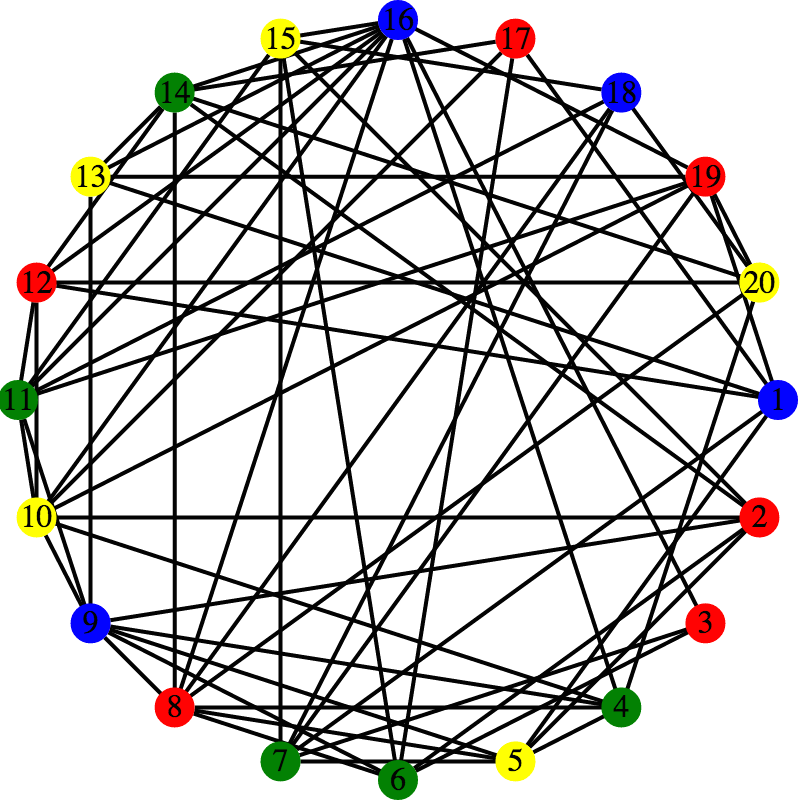
\includegraphics[width=0.5\columnwidth]{figures/web_graph}
	\caption{Sample Website Link Graph}\label{fig:web_graph}
\end{figure}

In addition to the link graph for the simulated side, textual content and images are also added to each page.  A subset of randomly generated images are included on each page simulating the  images that can be found in headers, footers or logos of a website.  Test content is also included in each page, using randomly generated lorem-ipsum.

Using this locally generated website, we ensure that our testing is not skewed by connection latency or other last mile problems that exist when testing across physical network infrastructure, isolating the latency to only that introduced by the processing of the CDN datacenter.  Additionally, it allows for the measurement of the number of requests that make it to the origin without having to add excessive tooling on the CDN servers.

\subsection*{Client}
To replicate real-world users, we create a number of client instances using docker containers. Each client browses to a page of the simulated website with a time delay of one second between each page, and each next page being randomly chosen from among the links of the current page. For a single page, each individual resource corresponds to a client request. Total number of client requests and PLT are calculated on the client. 

\subsection*{Server}
The general configuration of the servers within our tests has remained constant across implementations, with only the difference in logic for content fetching.  Servers are connected to a Redis node, which is used to store a set of all the servers to simplify the DHT generation and maintain a consistent hash table.  Redis’ publish/subscribe functionality is also used to broadcast bloom filter updates for each server on a fixed interval of 15 seconds.

For the sake of our tests, each server is considered to have “unlimited” capacity to store pages.  This was a design decision made to simplify initial implementation and due to the fact we are only caching content for a single website, as a single websites resources would not strain an actual CDN datacenter’s caching capabilities.  Further research and development will be done to support cache expiration and capacity limiting to be able to serve as a CDN for multiple websites, but it was not within the purview of this project. 

\begin{figure}[!h]
	\centering
	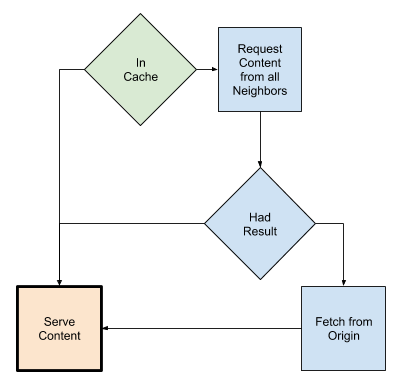
\includegraphics[width=0.7\columnwidth]{figures/cache_logic_before.png}
	\caption{Previous Implementation}
\end{figure}

Our initial server cache lookup implementation involved the following logic when processing requests. Given an initial request to a receiving server, the server checks to see if the content is in its local cache; if it is, it is returned directly.  If the content is not within the cache, parallel queries are made to each of the other members in the pool to see if they have the content.  If one of the neighbors has the requested content, the original server would cache it as well and return it to the client. Otherwise, the content is requested from the origin server, the result cached, and the response returned to the client. 

This design has multiple weak points even though it mirrors a standard distributed cache algorithm~\cite{mao2012cache}.  This style of naive requesting adds to the congestion of the backing datacenter and causes a fanout where each incoming request has the possibility of spawning O(n) internal queries, where n is the number of servers in the pool.  Additionally, this method duplicates the data across each server in the pool, which can be problematic when caching large amounts of content.

Our enhancement to naive flood requests is to have each server be aware of the neighboring cache contents using bloom filters in addition to using DHT logic to ensure cache content is only stored on a single server.  

The logic for processing incoming requests is as follows: first check if the receiving server is the designated owner of the content according to the DHT.  If so, and if the content requested is already in the cache, immediately return it; otherwise request the content from the origin server and cache the response.  If the receiving server is not the owner, the bloom filter of the owner is consulted to see if the content is cached on the owner.  If the owner does have the content, the content is requested  from them and returned it to the client. Otherwise a request by the receiving server is made to the origin server on the owner’s behalf, and the content is sent both to the owner to add to its cache and back to the client. 

For this design to work, bloom filters are broadcasted amongst the pool of servers on a fixed interval of 15 seconds.  This can lead to a delay in time in which despite having the content, pushes are being done to owners, up until the state of the owning server’s cache is broadcasted. Future work has been considered where this could be mitigated by adding an additional announcement to the pub-sub system that broadcasts when new content is added to a particular server, thus having less time in which the bloom filter is stale.

Each module is containerized in order to simplify the configuration required when evaluating aspects of this system.  Origin and Server modules are scaled behind the HAProxy load-balancer, which allows the even distribution of request load among the backing resources. The number of clients are a configurable parameter of the system, and can be scaled for testing. 

\begin{figure}[!h]
	\centering
	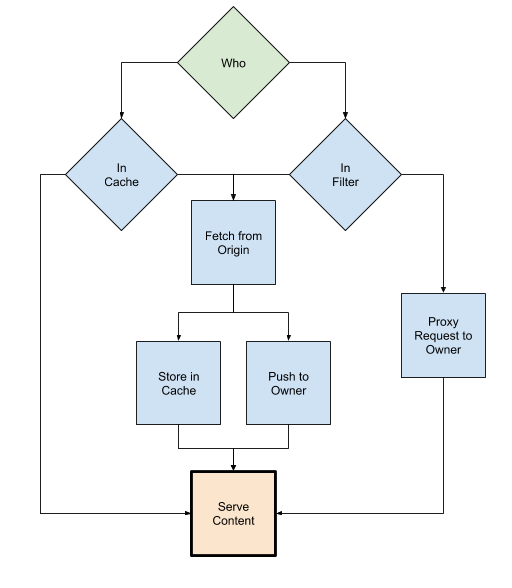
\includegraphics[width=0.7\columnwidth]{figures/cache_logic_after.png}
	\caption{DHT and Bloom Push Implementation}
\end{figure}

\section{Results}\label{sec:results}
To evaluate our system, we ran a suite of tests that simulated having one client to fifty-five clients, incremented in steps of two. This was done on both our pre-existing implementation of server fan out and our DHT/Bloom Push implementation.  This will allow us to compare the cache hit/miss ratios and PLT between the two implementations.

Below are the set of graphs from the preexisting fanout implementation showing the relationship between number of clients, hit and miss counts, and server to server requests. As seen in the Clients vs Datacenter Communications graph, an increase in client numbers correlates to an increase in cache misses. Furthermore, an increase in clients corresponds to a dramatic increase in PLT, seen in Figure 7, which we believe is caused by congestion within the datacenter, delaying the response times to client requests. 

\begin{figure}[!h]
	\centering
	\begin{subfigure}[b]{0.49\columnwidth}
		\centering
		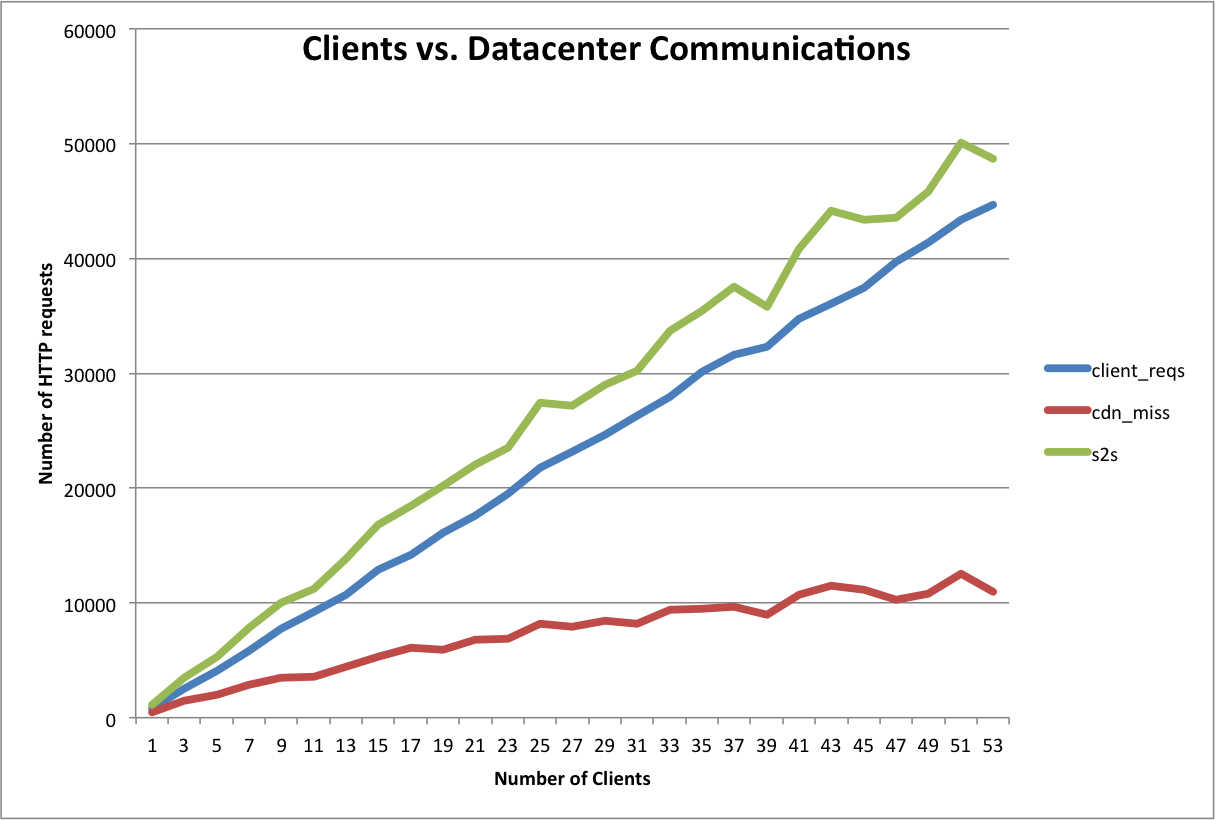
\includegraphics[width=\columnwidth]{figures/client-server.png}
	\end{subfigure}
	\begin{subfigure}[b]{0.49\columnwidth}
		\centering
		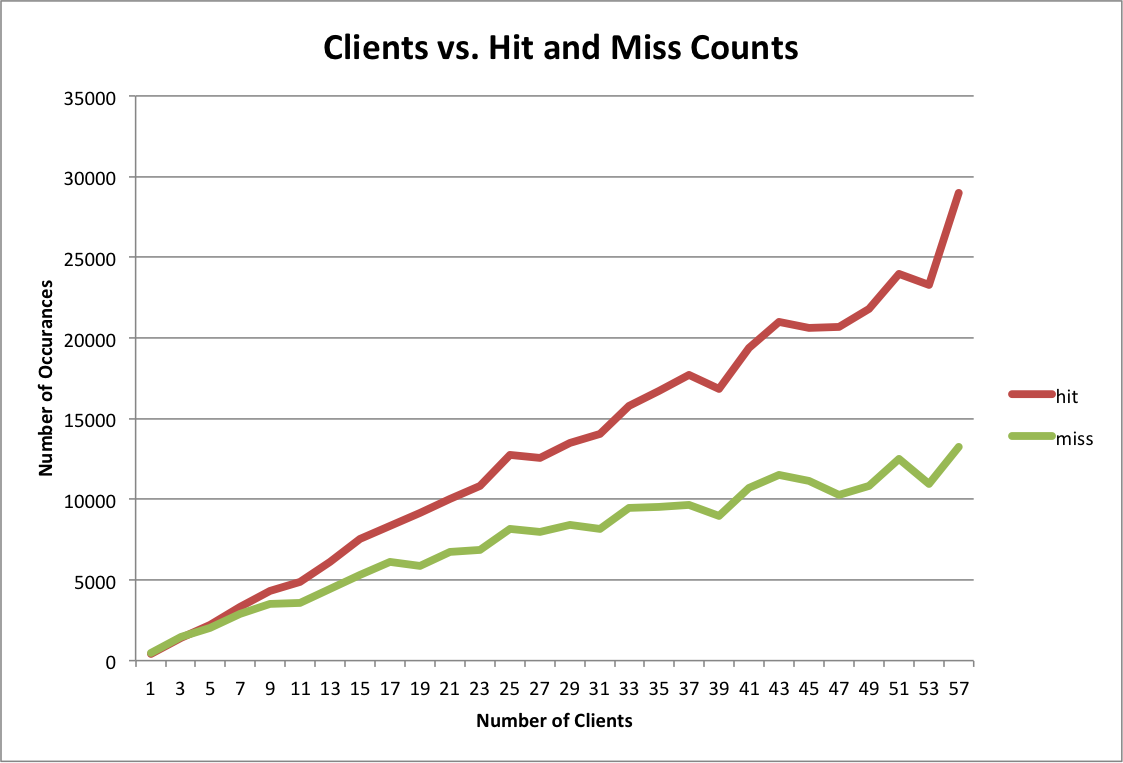
\includegraphics[width=\columnwidth]{figures/hit_miss_separate.png}
	\end{subfigure}
	\caption{Before}
\end{figure}

The set of graphs below show the same metrics gathered while using the DHT and Bloom Push system. The approximate number of client requests remains the same across all graphs. As expected, the Clients vs Datacenter Communications graph shows the number of server-to-server requests is dramatically reduced, going from a high of 50000 of the previous implementation, to a high of 24000 with DHT and Bloom Push, a reduction of over 50\%. This graphs also show a similar level of decrease in cache misses. 

\begin{figure}[!h]
	\centering
	\begin{subfigure}[b]{0.49\columnwidth}
		\centering
		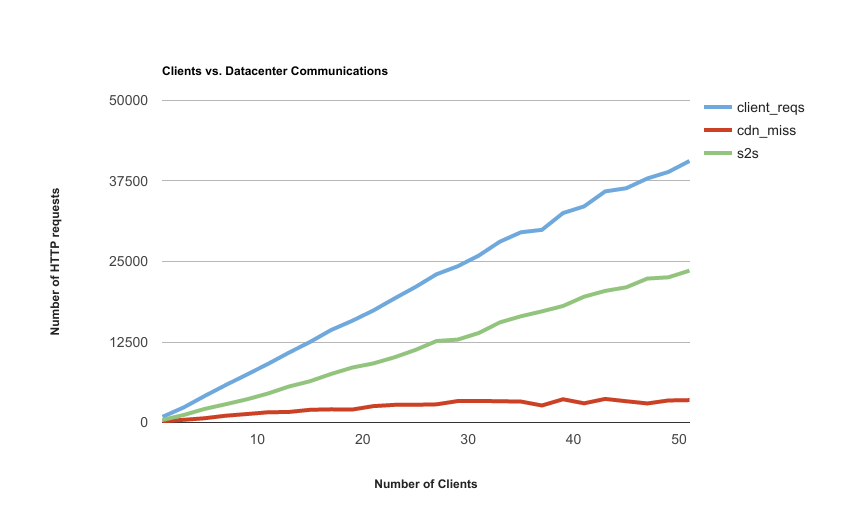
\includegraphics[width=\columnwidth]{figures/client-server_1.png}
	\end{subfigure}
	\begin{subfigure}[b]{0.49\columnwidth}
		\centering
		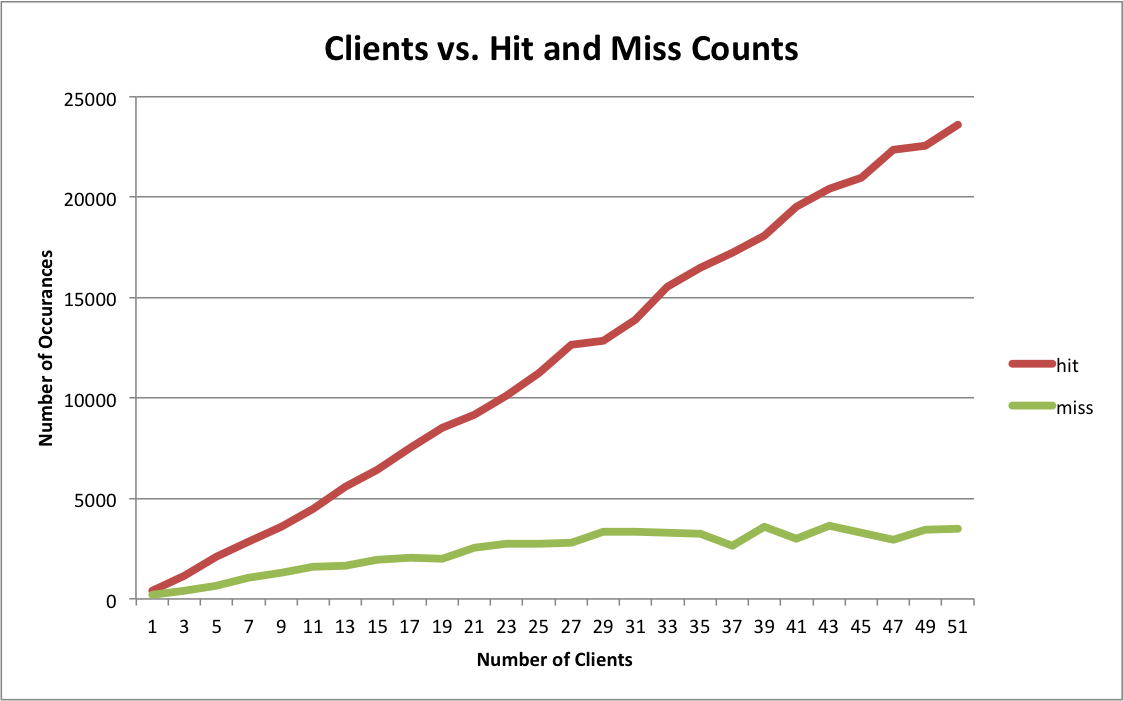
\includegraphics[width=\columnwidth]{figures/hit_miss_separate_1.png}
	\end{subfigure}
	\caption{After}
\end{figure}

The final set of graphs are below, showing the previous Hit/Miss Ratio and PLT vs those gathered with the DHT and Bloom Push system. The Hit/Miss Ratio graph shows a difference of 2 to 7.5, in favor of the new system, confirming success of the system in reducing cache misses while scaling to greater numbers of clients. However, we did not see the PLT decrease as expected; unfortunately, that metric actually worsened, especially as the number of clients increased past 30 and for the high percentiles.

Further experimentation led us to believe that the mistake in our logic was having only a single server being responsible for a certain subset of data, meaning the load on that server became disadvantageous as the number of clients increased. Ideally, given a fixed cache size and multiple websites, we could have multiple servers responsible for a subset of data, and then query the smaller set of servers, instead of all servers as in our first implementation, and a single server as in our current implementation. 

\begin{figure}[!h]
	\centering
	\begin{subfigure}[b]{0.49\columnwidth}
		\centering
		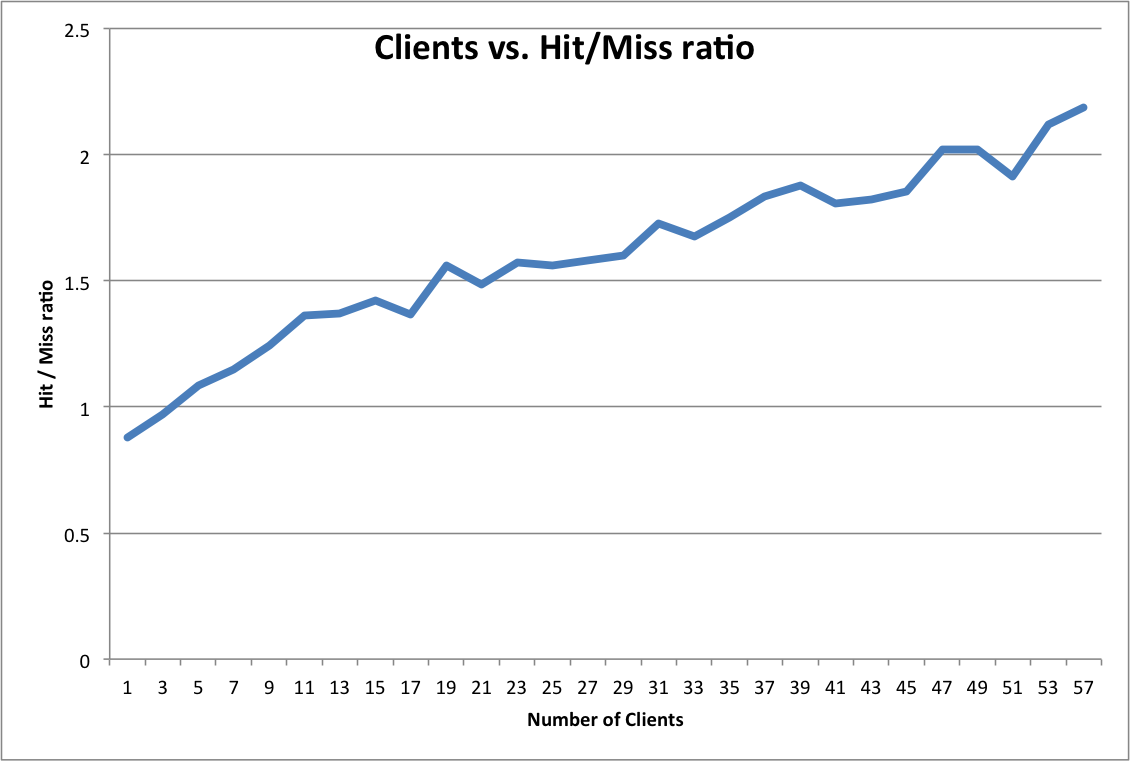
\includegraphics[width=\columnwidth]{figures/hit_miss.png}
	\end{subfigure}
	\begin{subfigure}[b]{0.49\columnwidth}
		\centering
		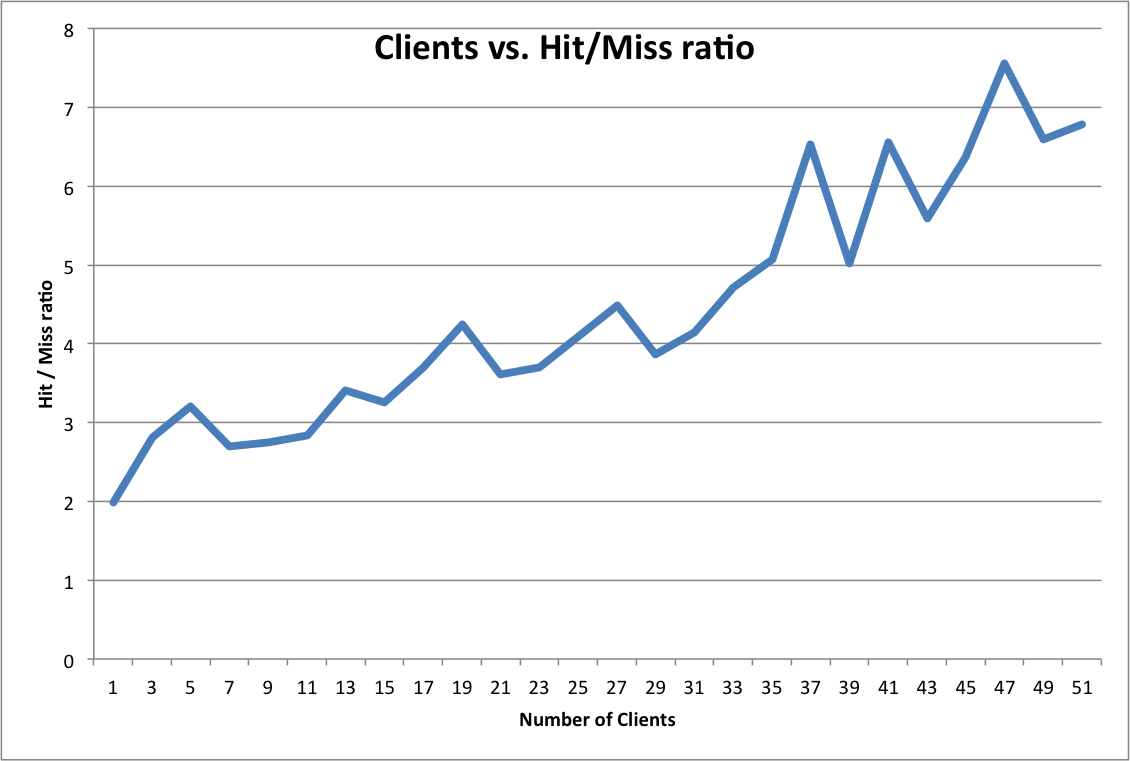
\includegraphics[width=\columnwidth]{figures/hit_miss_1.png}
	\end{subfigure}
	\caption{Hit/Miss Comparison}
\end{figure}

\begin{figure}[!h]
	\centering
	\begin{subfigure}[b]{0.49\columnwidth}
		\centering
		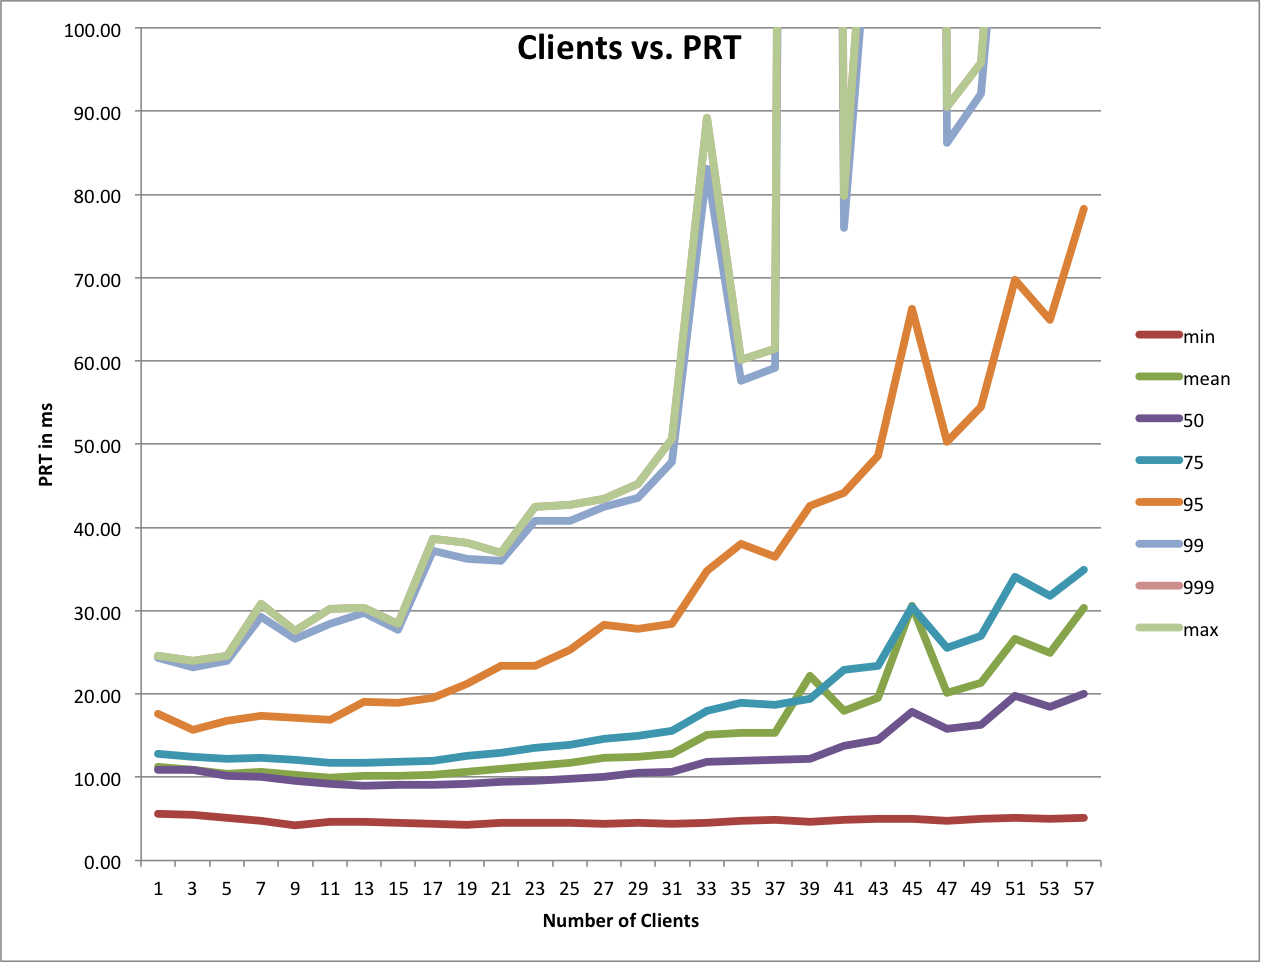
\includegraphics[width=\columnwidth]{figures/render.png}
	\end{subfigure}
	\begin{subfigure}[b]{0.49\columnwidth}
		\centering
		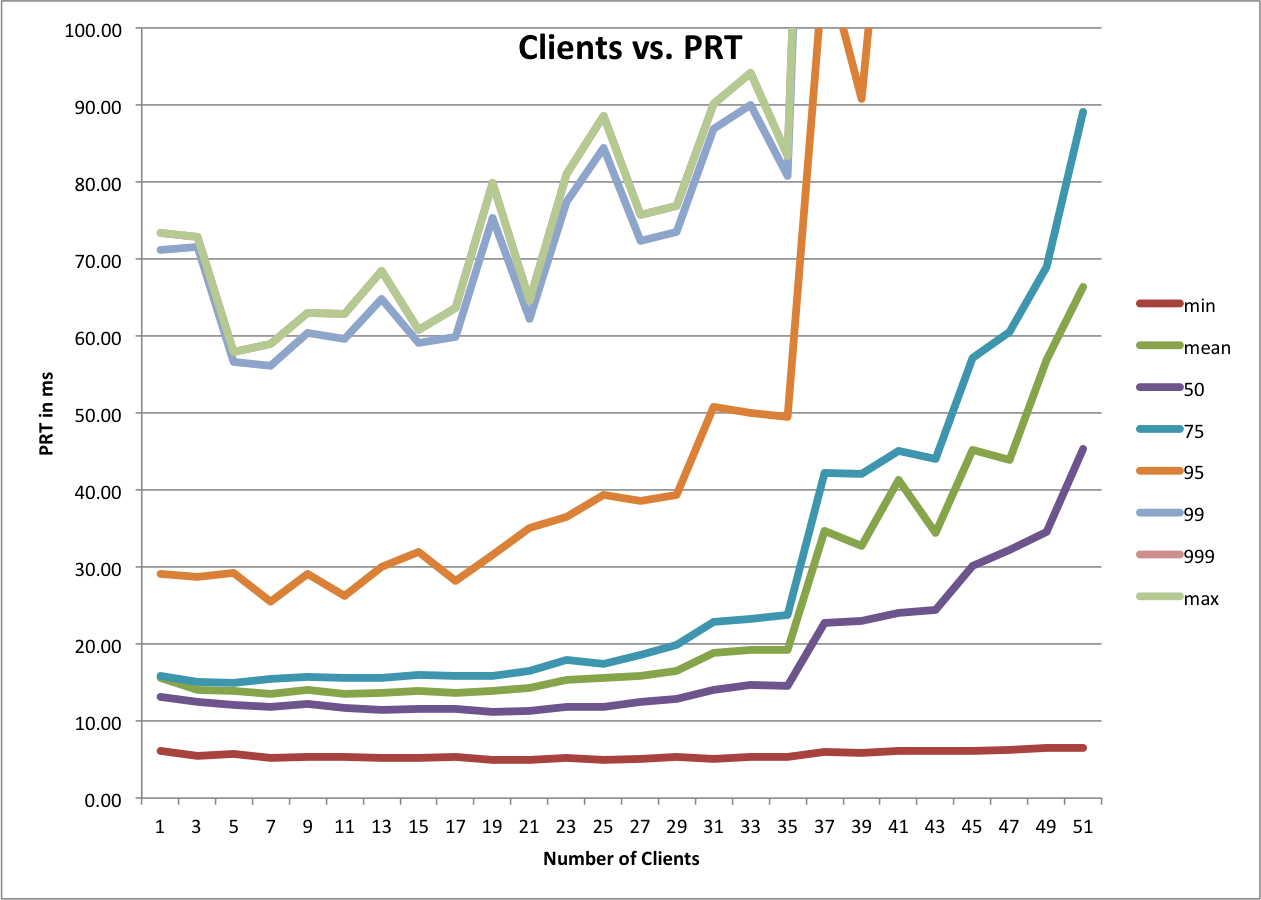
\includegraphics[width=\columnwidth]{figures/render_1.png}
	\end{subfigure}
	\caption{PLT Comparison}
\end{figure}


%In Figure~\ref{fig:abc} ...

%\begin{figure}[!h]
%	\centering
%	\begin{subfigure}[b]{0.49\columnwidth}
%		\centering
%		\includegraphics[width=\columnwidth]{img/abc.png}
%		\caption{abc}
%		\label{fig:abc}
%	\end{subfigure}
%	\begin{subfigure}[b]{0.49\columnwidth}
%		\centering
%		\includegraphics[width=\columnwidth]{img/sdf.png}
%		\caption{sdf}
%		\label{fig:sdf}
%	\end{subfigure}
%	\caption{abc + sdf}
%\end{figure}


\section{Conclusion}\label{sec:conclusion}
In this paper we offer a brief overview of CDNs and the use of Distributed Hash Tables and Bloom Filters in their infrastructure. We present a new system, Bloom Push, created using state of the art technologies that replicates the functionality of a CDN datacenter and incorporates a novel approach to using Bloom Filters and server push in conjunction to successfully reduce the amount of cache misses in our system. We have proved our system is scalable with increasing numbers of clients, but did not meet our goal of proving the Bloom Push system could decrease Page Load Time. 

For the future work on the system, we wish to extend the bloom push improvements by duplicating data on a subset of servers within the pool, allowing for reduced load on any individual cache within the system.  Also, it may be a useful extension to split the caching logic from the content requesting logic to separate modules to improve scalability and logic isolation.  NATS is another pub-sub server and it may be worth migrating due to increased performance over Redis; this could allow for individual broadcasting of adding items in a cache rather than broadcasting bloom filters on an interval which adds communication but reduces memory consumption from the cache.

\bibliographystyle{plain}
\bibliography{cdn}

\end{document}
